\subsection{Dataset}
We have conducted experiments on the following datasets(Mainly For Phase 1):
\begin{center}
\begin{tabular}{| l | c |}
  \hline                        
  Dataset Name & Advogato  \\ \hline
  Largest conn compo & 5054  \\ \hline
  Size & 6551 vertices  \\ \hline
  Volume & 51332 edges \\ \hline
\end{tabular}
\end{center}

In out final experiment suit, a more large and diverse datasets from different domains will be explored. The tentative source of experiment dataset are listed below:
\begin{description}
	\item{{\bf SNAP:}}{It has abundant data about social network, we plan to conduct triangle counting, pagerank, radius computing experiment which will reveal the underlying feature of large graphs and spot strange graphs.}
	\item{{\bf Konect:}}{Konect has more diverse datasets compared to SNAP, like citation network. It's a good target to analyze features of non-social networks, we will examine whether such networks follow power law by generating degree distribution, etc.}
\end{description}

We also calculated statistics about the weakly connected components in table \ref{table:wcc}.We compute radius for every node in Advogato dataset, the result is in table \ref{table:radius}:

\subsection{Task 1: Degree distribution}

\subsubsection{Description}
We conduct 5 experiments on large scale graph data(all with more than 1 million nodes). The details of each dataset is as follows: \\

\begin{center}
\begin{tabular}{| c | c | c |}
    \hline
    name & nodes & edges \\ \hline
    Roadnet-ca & 1,965,206 & 5,533,214 \\ \hline
    Roadnet-PA & 1,088,092 & 3,083,796 \\ \hline
    Roadnet-TX & 1,379,917 & 3,843,320 \\ \hline
    wiki-Talk & 2,394,385 & 5,021,410 \\ \hline
    Youtube & 1,134,890 & 2,987,624 \\ \hline
\end{tabular}
\end{center}


Following(Figure \ref{t1:plot}) are the rank-frequency plots of each dataset, (a)(b) shows the in degree and out degree out Wikitalk. (c) is Roadnet-Ca. (d) is Roadnet-PA. (e) is Roadnet-TX. (f) is Youtube. 

\subsubsection{Plots}

\begin{figure}[!htbf]
\begin{center}
\begin{tabular}{c c c}
     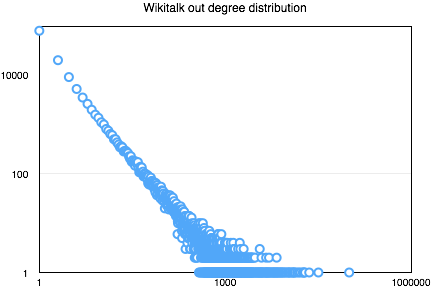
\includegraphics[width=0.3\textwidth]{FIG/t1_wiki_in.png} &
     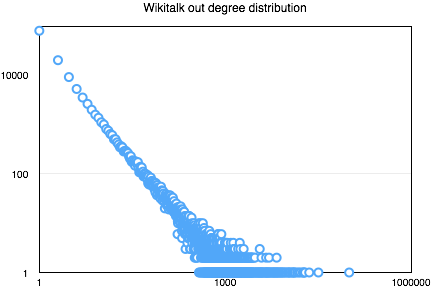
\includegraphics[width=0.3\textwidth]{FIG/t1_wiki_out.png} & 
     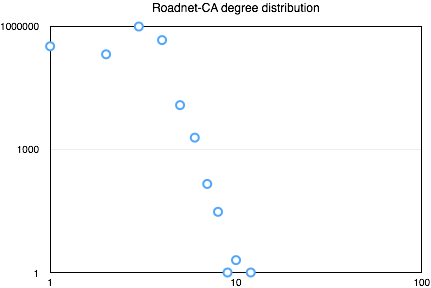
\includegraphics[width=0.3\textwidth]{FIG/t1_ca.png}\\
    (a) & (b) & (c) \\
     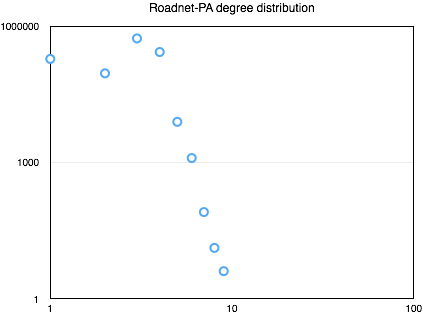
\includegraphics[width=0.3\textwidth]{FIG/t1_pa.png} & 
     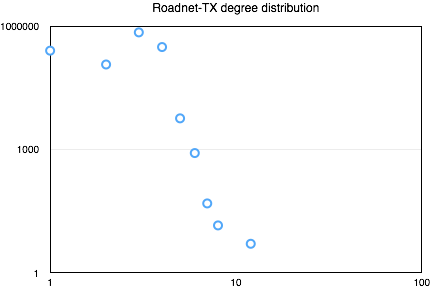
\includegraphics[width=0.3\textwidth]{FIG/t1_tx.png} & 
     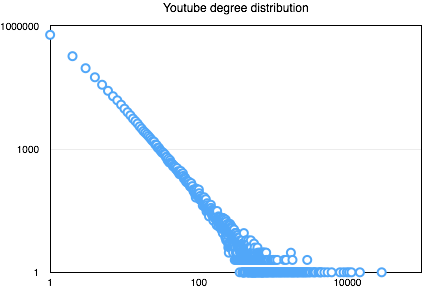
\includegraphics[width=0.3\textwidth]{FIG/t1_youtube.png} \\
     (d) & (e) & (f) \\
\end{tabular}
\caption{In degree distribution (a) and out degree distribution (b) of Wikitalk (c) Roadnet-CA, (d) Roadnet-PA (e) Roadnet-TX (f) Youtube}
\label{t1:plot}
\end{center}
\end{figure}

\subsubsection{Observation}
As we can observe, that most \emph{social network} exhibit perfect power law in degree distribution. It aligned with our intuition. While for the series of Roadnet dataset, we can not observe obvious power law. So maybe we can conclude that not all graphs have power law property in it. Some datasets like roadnet, involves a lot of human design, is less \emph{chaotic} than ordinary graphs.

\subsection{Task 2: Pagerank}

\subsection{Task 3: Weakly Connected Component}
In this experiment, we run weakly connected component in several datasets of various size.

\subsubsection{Plot}
We draw size-frequency plot in log-log scales.
\begin{figure}[h]
\begin{center}
     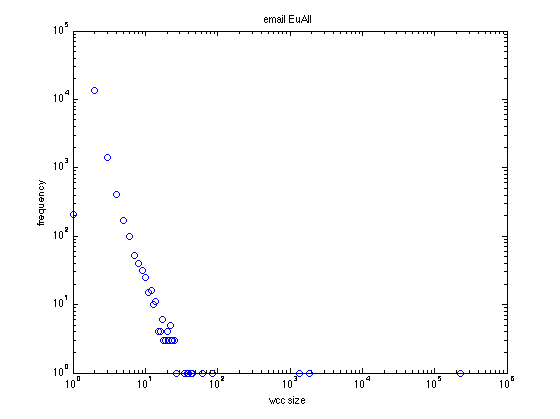
\includegraphics[width=0.8\textwidth]{FIG/t3_email_euall.png} 
\caption{Email-EuAll }
\label{t3:1}
\end{center}
\end{figure}

\begin{figure}[h]
\begin{center}
\begin{tabular}{cc}
     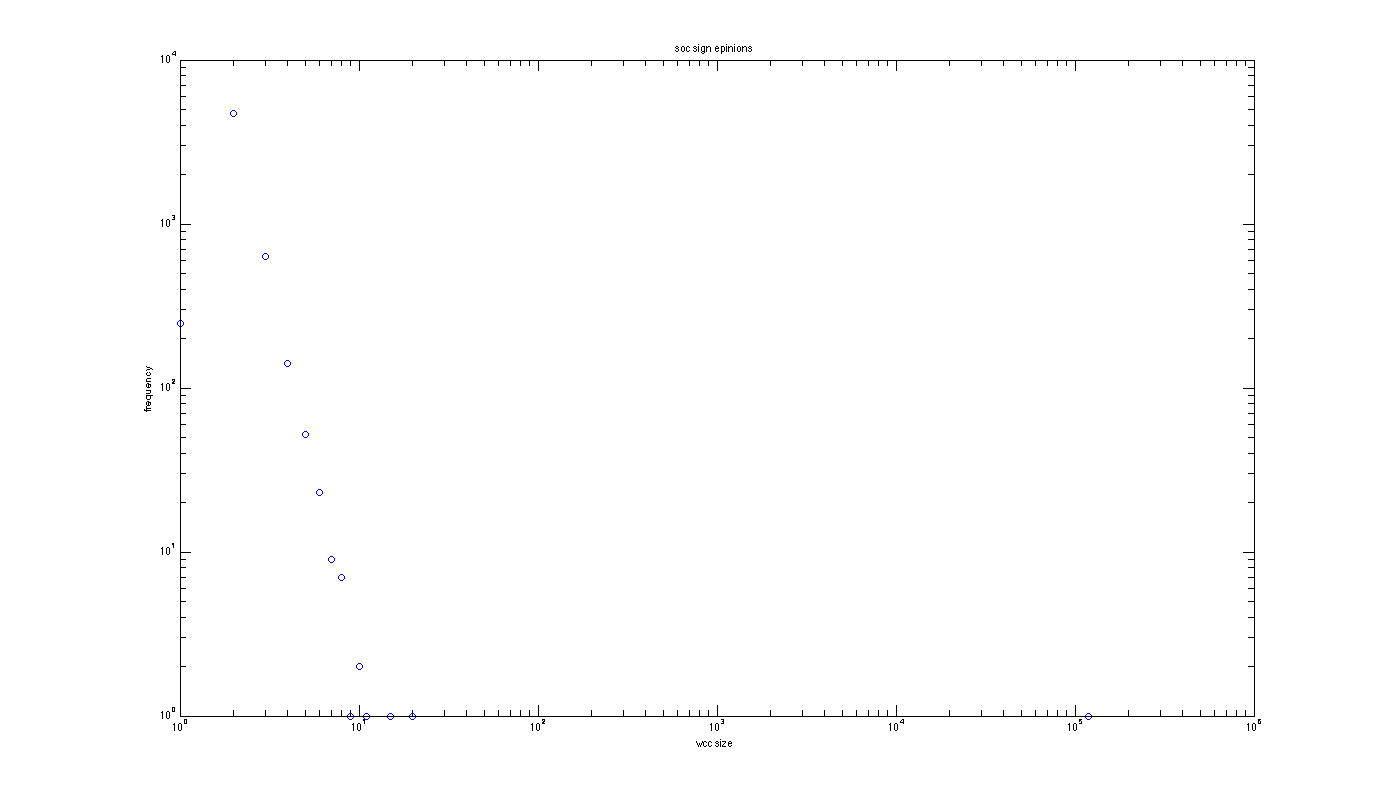
\includegraphics[width=0.8\textwidth]{FIG/t3_soc_sign_epinions.png} 
\end{tabular}
\caption{Soc-Sign-Epinions}
\label{t3:2}
\end{center}
\end{figure}


\begin{figure}[h]
\begin{center}
     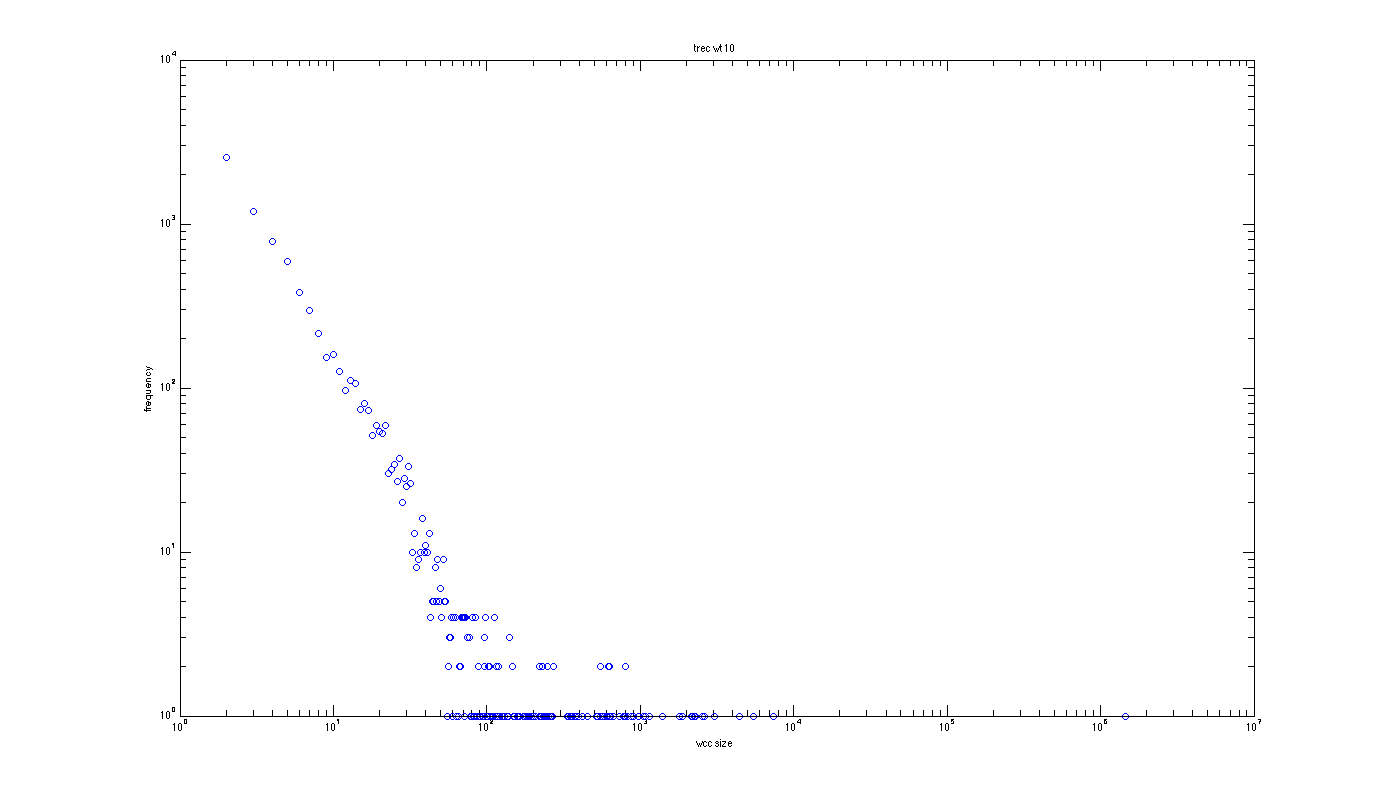
\includegraphics[width=0.8\textwidth]{FIG/t3_trec_wt10.png} 
\caption{Trec-wt10g}
\label{t3:3}
\end{center}
\end{figure}


\begin{figure}[h]
\begin{center}
     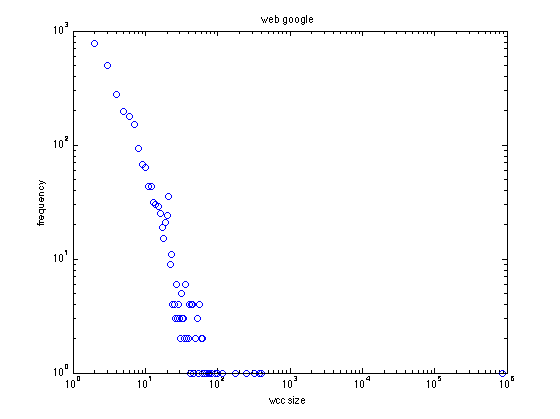
\includegraphics[width=0.8\textwidth]{FIG/t3_web_google.png} 
\caption{Google Web Graph}
\label{t3:4}
\end{center}
\end{figure}


\begin{figure}[h]
\begin{center}
     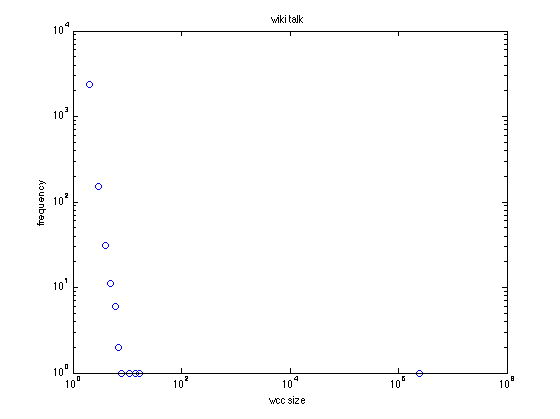
\includegraphics[width=0.8\textwidth]{FIG/t3_wiki_talk.png} 
\caption{Wiki Talk}
\label{t3:5}
\end{center}
\end{figure}

\subsubsection{Observation}
1. From the log-log scale frequency-size plot, we find that generally frequency-size follows the power law. Connected components of small sizes tend to occur more often those of larger sizes.

2. In all the plots, there is a giant connected component that contains the majority of nodes in the graph. 






\subsection{Task 4: Radius of Every Node}

\subsubsection{Experiment on large datasets}
In this experiment, we run our radius algorithm in several large datasets. The statistics of these datasets are presented in Table \ref{t4:table1}

\begin{table}[!htbf]
\caption{Datasets Statistics}
\begin{center}
\begin{tabular}{|c|c|c|c|}
\hline \hline
dataset & number of vertices & number of edges & diameter \\
\hline
DBLP co-authorship network & 317080  & 1049866  & 21  \\
Epinions social network & 131828  & 841372  & 14  \\
Amazon product co-purchasing network & 334863 & 925872 & 44 \\
EU email communication network & 265214 & 420045 & 14 \\
Google web graph & 875713 & 5105039 & 21 \\
Youtube social network & 1134890 & 2987624 & 20 \\
\hline
\end{tabular}
\end{center}
\label{t4:table1}
\end{table}%


\begin{figure}[!htbf]
\begin{center}
     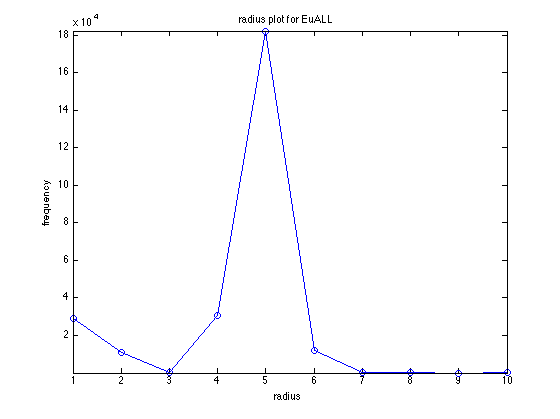
\includegraphics[width=0.8\textwidth]{FIG/t4_email.png} 
\caption{EU Email Communication }
\label{t4:1}
\end{center}
\end{figure}

\begin{figure}[!htbf]
\begin{center}
\begin{tabular}{cc}
     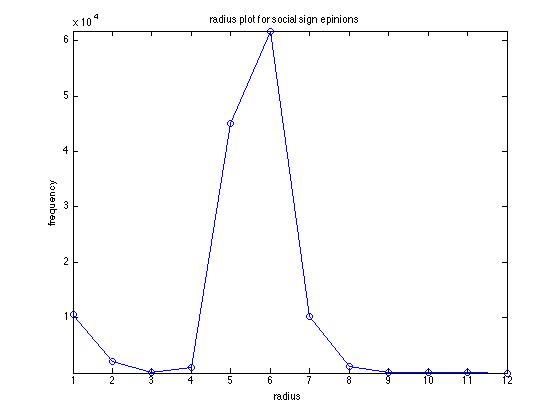
\includegraphics[width=0.8\textwidth]{FIG/t4_epinions.png} 
\end{tabular}
\caption{Epinions social network}
\label{t4:2}
\end{center}
\end{figure}


\begin{figure}[!htbf]
\begin{center}
     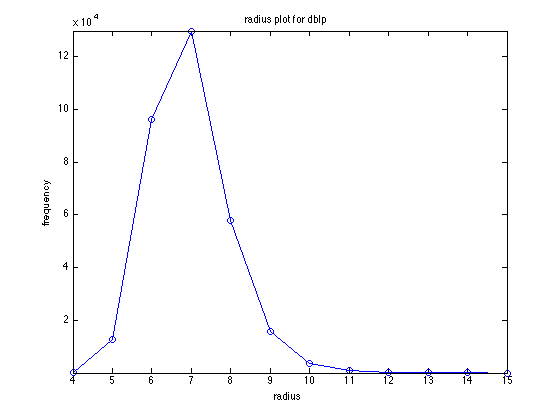
\includegraphics[width=0.8\textwidth]{FIG/t4_dblp.png} 
\caption{DBLP co-authorship network}
\label{t4:3}
\end{center}
\end{figure}


\begin{figure}[!htbf]
\begin{center}
     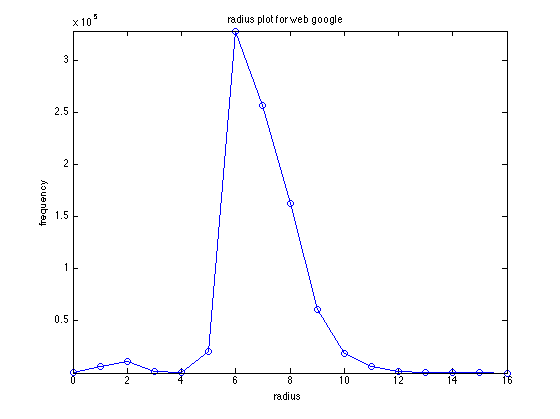
\includegraphics[width=0.8\textwidth]{FIG/t4_google.png} 
\caption{Google Web Graph}
\label{t4:4}
\end{center}
\end{figure}


\begin{figure}[!htbf]
\begin{center}
     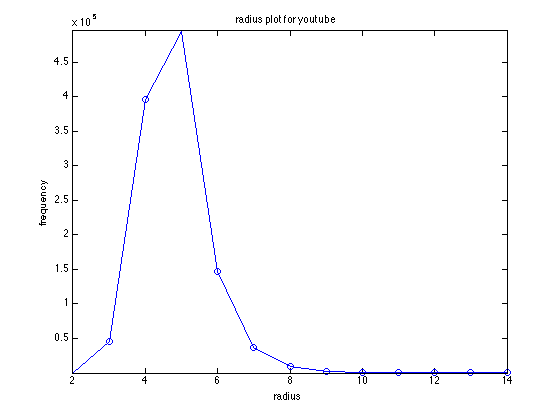
\includegraphics[width=0.8\textwidth]{FIG/t4_youtube.png} 
\caption{Youtube Social Network}
\label{t4:5}
\end{center}
\end{figure}

\begin{figure}[!htbf]
\begin{center}
     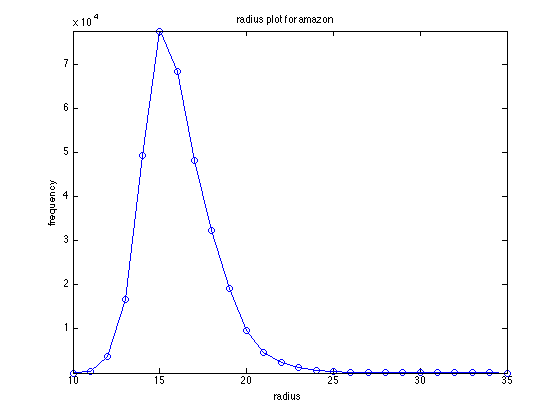
\includegraphics[width=0.8\textwidth]{FIG/t4_amazon.png} 
\caption{Amazon product co-purchasing networkk}
\label{t4:6}
\end{center}
\end{figure}


 
\subsubsection{Observation}
1. Radius Distribution: From the above plot, we find radius distribution of these graphs either tend to be single-modal, for example, EU Email Communication graph in figure \ref{t4:1} and Epinions Social Network in figure \ref {t4:2}, or bi-modal like DBLP co-authorship network in figure \ref{t4:3} and Youtube Social Network in figure \ref{t4:5}.

2. Relationship to the connected component: So why radius tend to be distributed like this, we guess it's somehow related to the connectivity of the graph. Therefore we take a look back to the statistics we got from task3. We find that the graphs that has a single-modal shape radius distribution are fully or almost fully connected. The graphs that has bi-modal radius distribution are not that well connected, For most nodes that appear in the Giant Connected Component(GCC), they tend to have a higher radius value, specifically the smaller radius value it has, the more centric it is in the GCC. On the other hand, The first peak in the radius distribution represent those disconnected components.

\subsubsection{Proof of Correctness}
Since the algorithm we use is an approximate algorithm, it's hard for us to verify the validity of our algorithm accurately. But we still try the algorithm on both small, large and synthetic datasets to demonstrate its validity.  
First we test the algorithm on the synthetic tiny dataset consisting of only 10 nodes and 8 edges. It accurately compute the radius of every node.
 
Then we test our algorithm on small datasets of several thousands of nodes, the experiment result are showed in Table \ref{table:small}, we can see that our algorithm can get a closer estimate of diameter.

\begin{table}[!htbf]
\caption{Radius Experiment on Small Datasets}
\begin{center}
\begin{tabular}{|c|c|c|c|c|}
\hline \hline
dataset & nodes & edges & real diameter & estimated diameter \\
\hline
Enron email network & 36692 & 183831 & 11 & 11 \\
High Energy Physics & 12008 & 118521 & 13 & 12 \\
Advogato Trust Network & 6551 & 51332 & 9 & 9 \\
\hline
\end{tabular}
\end{center}
\label{table:small}
\end{table}%

For large dataset we run in last section, the estimated diameter is still bounded by real diameter, but the estimation is no longer that close. This can be explained by the approximation nature of the algorithm we use. The Flajolet-Martin string we generate for every node is not unique, and as the number of nodes grows larger, the uniqueness of a node that a Flajolet-Martin string can represent is weakened. Therefore, for graph with larger size, the estimation might become less accurate.







\subsection{Task 5: Eigenvalue/Singular value}


\subsection{Task 6: Belief Propagation}

\subsubsection{Experiment on large datasets}
In this experiment, we run our radius algorithm in several large datasets. The statistics of these datasets are presented in Table \ref{t5:table1}

\begin{table}[!htbf]
\caption{Datasets Statistics}
\begin{center}
\begin{tabular}{|c|c|c|}
\hline \hline
dataset & number of vertices & number of edges \\
\hline
DBLP co-authorship network & 317080  & 1049866  \\
Epinions social network & 131828  & 841372  \\
Amazon product co-purchasing network & 334863 & 925872 \\
EU email communication network & 265214 & 420045 \\
Google web graph & 875713 & 5105039 \\
Youtube social network & 1134890 & 2987624 \\
\hline
\end{tabular}
\end{center}
\label{t5:table1}
\end{table}%

Similar to semi-supervised learning, belief propagation algorithm require the graph to be partially labeled.  However, we don't have such information. Therefore, in this experiment, we randomly assign the prior belief for all nodes. Specifically, we randomly assign 25 percent of the nodes with positive label, i.e. positive prior belief, and 25 percent of other nodes with negative label, i.e. negative prior belief, and the rest with zero belief, meaning that we don't have prior knowledge for these nodes. Then we conduct FABP algorithm on these datasets, the result are shown in Table \ref{t5:table2} .

\begin{table}[!htbf]
\caption{BP Statistics}
\begin{center}
\begin{tabular}{|c|c|c|c|}
\hline \hline
dataset & positively labeled & negatively labeled & non labeled  \\
\hline
DBLP co-authorship network & 134139  & 136636  & 46305 \\
Epinions social network & 53968  & 52796  & 25064 \\
Amazon product co-purchasing network & 143796 & 144796 & 46271 \\
EU email communication network & 100619 & 109674 & 54921 \\
Google web graph & 379568 & 376325 & 119820 \\
Youtube social network & 450084 & 457956 & 226850 \\
\hline
\end{tabular}
\end{center}
\label{t5:table2}
\end{table}%

 
\subsubsection{Observation}
1. By applying Belief Propagation algorithm on these graphs, most of the unlabeled nodes are successfully assigned either positive or negative belief.

2. We find that for some graphs, larger proportions of nodes gets labeled than other graph. For example, in DBLP co-authorship network and amazon product co-purchasing network,  about 85\%  of the nodes get labeled. While for like Epinions social network and EU emali communication network, only 75\% of the nodes get labeled. Once again, we look back at the connectivity of the graph to find the probable cause. We observed that, graph that is well connected is easier to get more nodes assigned with labels. This observation makes sense in that 'beliefs' can be easier to propagate in well connected graphs than those grape with many disconnected components.

\subsubsection{Proof of Correctness}
As mentioned it the previous section, we don't have any labels for these large datasets, therefore we verify the result according to statistics we get in the last section. We can see that the proportion with positive labels and negative labels are approximately same, which resembles the label distribution with our prior belief. 







\subsection{Task 7: Triangle Counting}
According to the algorithms in \cite{tsourakakis2008fast}, we know that the number of triangles in a network is propotional to the sum of eigenvalue of its adjency matrix, which is $\frac{\sum_{i}\lambda_{i}^{3}}{6}$. Figure \ref{t7:timedata} shows the running time of global triangle counting with regards to the size of graph. We can see that as the size of graph increases, the running time also grows nearly linearly with the size. For the largest graph, which is Roadnet-PA, it runs nearly for an hour to complete. However, the predicted result for Roadnet-PA is unsatisfactory. We conduct both global and local triangle counting, all the data is listed as follows.

\subsubsection{Plots}
Table \ref{t7:timedata} lists run time of global triangle counting. Table \ref{t7:globalpredict} lists the predicted triangle count of each dataset. Figure \ref{t7:globaltime} plots the run time on each dataset. Figure \ref{t7:local} plots the rank-frequency plot of local triangle count on each dataset. 

\begin{table}
\begin{center}
\begin{tabular}{ | c | c | }
    \hline
    graph size & run time(seconds) \\ \hline
    7115 & 45.199s \\ \hline
    36692 & 72.76 \\ \hline
    82168 & 596.046 \\ \hline
    334863 & 1288.703 \\ \hline
    1088092 & 2980.985 \\ \hline
\end{tabular}
\end{center}
\caption{Task 7 run time(global)}
\label{t7:timedata}
\end{table}

\begin{table}
\begin{center}
\begin{tabular} {| c | c | c | c | }
    \hline
    dataset & size & predict & truth \\ \hline
    wiki-Vite & 7115 & 661282 & 608389 \\ \hline
    Enron-email & 36692 & 276757 & 727044 \\ \hline
    slash-dot & 82168 & 1294037 & 602592 \\ \hline
    Amazon-com & 334863 & 13904 & 667129 \\ \hline
    Roadnet-PA & 1088092 & 55.95 & 67150 \\ \hline
\end{tabular}
\end{center}
\caption{Predicted triangle count(global)}
\label{t7:globalpredict}
\end{table}

\begin{figure}[!htbf]
\begin{center}
\begin{tabular}{c}
     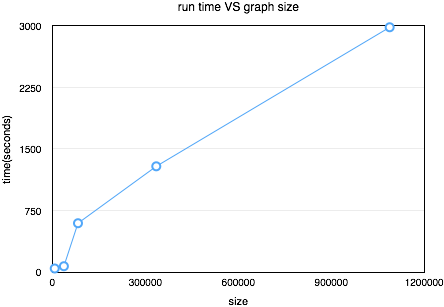
\includegraphics[width=0.8\textwidth]{FIG/t7_time.png}
\end{tabular}
\caption{Task 7: Run time VS graph size(global)}
\label{t7:globaltime}
\end{center}
\end{figure}

\begin{figure}[!htbf]
\begin{center}
\begin{tabular}{cc}
     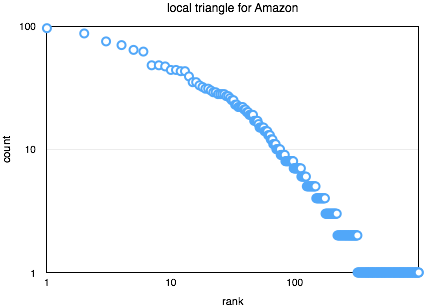
\includegraphics[width=0.4\textwidth]{FIG/t7_amazon.png} &
     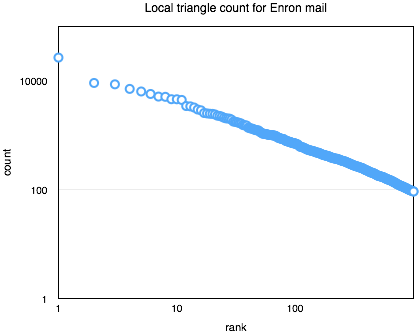
\includegraphics[width=0.4\textwidth]{FIG/t7_enron.png} \\
     (a) & (b) \\
     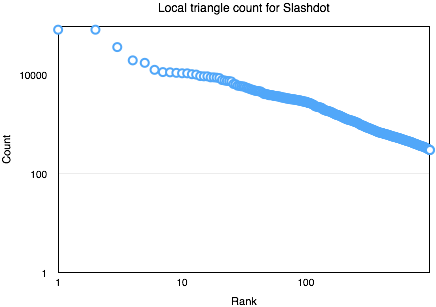
\includegraphics[width=0.4\textwidth]{FIG/t7_slashdot.png} &
     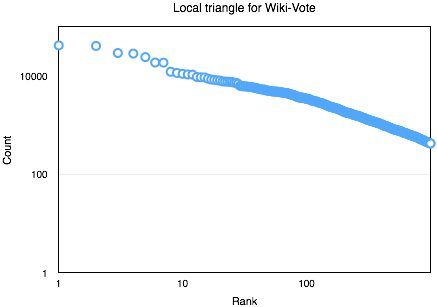
\includegraphics[width=0.4\textwidth]{FIG/t7_wikivote.png} \\
     (c) & (d) \\
     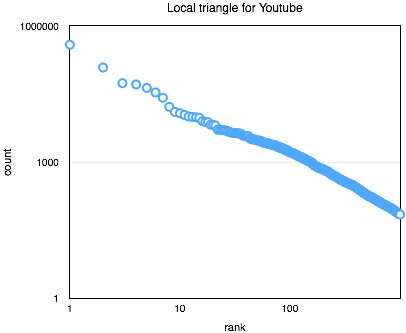
\includegraphics[width=0.4\textwidth]{FIG/t7_youtube.png} & \\
     (e)
\end{tabular}
\caption{Local triangle counting. (a) Amazon (b) Enron Mail (c) Slashdot (d) Wiki Vote (e) Youtube}
\label{t7:local}
\end{center}
\end{figure}

\subsubsection{Observation}
According to Figure \ref{t7:local}, we can see that the rank-frequency plot of local triangle count also follows power law. And we can observe that the run time grows nearly linearly with the graph size. 


\begin{table}
\begin{center}
\begin{tabular}{| l | c |}
  \hline                        
  Size of WCC & Count  \\ \hline
  1 & 1384  \\ \hline
  2 & 55  \\ \hline
  3 & 1 \\ \hline
  5054 & 1 \\ \hline  
\end{tabular}
\caption{Statistics about Weakly connected components}
\label{table:wcc}
\end{center}
\end{table}

\begin{table}
\begin{center}
\begin{tabular}{| l | c |}
  \hline                        
  radius & number of vertices  \\ \hline
  0 & 1896  \\ \hline
  1 & 84  \\ \hline
  2 & 11 \\ \hline
  3 & 7 \\ \hline  
  4 & 634 \\ \hline  
  5 & 2194 \\ \hline  
  6 & 826 \\ \hline  
  7 & 117 \\ \hline  
  8 & 13 \\ \hline
  9 & 2 \\ \hline   
\end{tabular}
\caption{statistics about radius}
\label{table:radius}
\end{center} 
\end{table}

\begin{figure}[htbf]
\begin{center}
     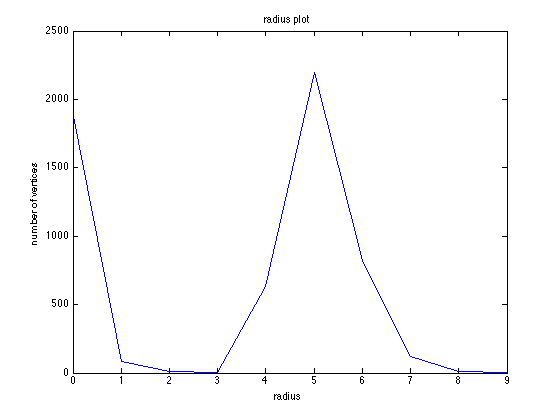
\includegraphics[width=0.6\textwidth]{FIG/radius.png}
\caption{Radius Plot}
\label{fig:radius}
\end{center}
\end{figure}

\subsection{Broad Spectrum Analysis}
We apply our proposed graph mining algorithms to several real-world graph datasets from KONECT project to find global patterns and detect strange behaviors. In the following, we'll first describe the dataest then discuss  what we observe. 

\begin{description}
	\item{{\bf Route Views\cite{konect:2013:as20000102, konect:DBLP}:}}{This is an undirected network of autonomous systems of the Internet connected with each other. Nodes are autonomous systems (AS), and edges denote communication. The network contains loops. It contains 6,474 vertices and 13,895 edges.}
	\item{{\bf DBLP\cite{konect:2013:dblp-cite, konect:DBLP}:}}{This is the citation network of DBLP, a database of scientific publications such as papers and books. Each node in the network is a publication, and each edge represents a citation of a publication by another publication. In other words, the directed edge (A to B) denotes that publication A cites publication B. Publications are allowed to cite themselves, and therefore the network contains loops. It contains 12,495 vertices and 49,793 edges.}
\end{description}

\begin{figure}[htbf]
\begin{center}
\begin{tabular}{cc}
     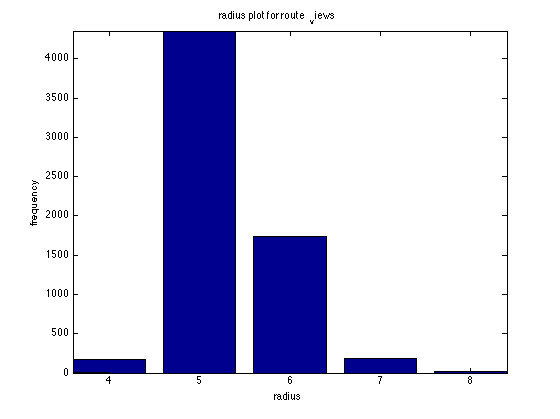
\includegraphics[width=0.4\textwidth]{FIG/route_radius.png} &
     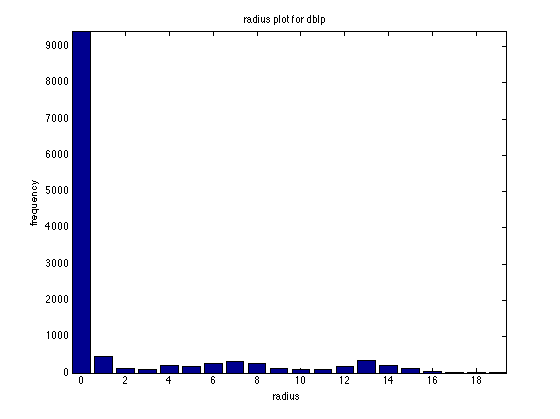
\includegraphics[width=0.4\textwidth]{FIG/dblp_radius.png} \\
    (a) & (b) 
\end{tabular}
\caption{Radius plot for Route Views (a) and Radius plot for DBLP (b)}
\label{fig:radius_plot}
\end{center}
\end{figure}

The radius plot for dataset are shown in figure \ref{fig:radius_plot}. 

From radius distribution of route views, we can see that all the vertices has radius more than 3. And since this is a connected graph (from the result we got by applying connected component algorithm), we can conclude that vertices(Autonomous Systems) with smaller radius plays a more centric role in the graph where most other vertices have direct or indirect communication (within very few hops) with. We find very few vertices with radius 4 are in the center of the graph, then most of the vertices with radius 5 are surrounding these centric vertices. Then the number of vertices decrease exponetialy as the radius grows. And finally, very few vertices (less than 20) are in the margin of the entire AS networks.  

For another graph DBLP, we observe strange behaviors. In this radius distribution, we observe that the great majority of the vertices have 0 radius, which means these papers didn't cite any other papers. We can only explain this observation by assuming all the cited papers of all those 9000 papers are not within this dataset. For other radius value, we don't observe apparent power law but rather more or less uniform distribution. However, in an exact or more complete citation graph, we should see several few popular papers pointing to each other, and has rather small radius, and most other less famous papers has longer citation path (larger radius). Therefore, we can conclude that this is a small sub-graph that don't capture the significant characteristic of a complete citation graph.


